\documentclass[10pt,conference,compsocconf]{IEEEtran}

\usepackage{hyperref}
\usepackage{graphicx}	% For figure environment


\begin{document}
\title{Higgs Boson Machine Learning Challenge}

\author{
  Sebastien Savidan, Jean Gschwind, Tristan Besson\\
  \textit{Machine Learning Course, EPFL, Switzerland}
}

\maketitle

\begin{abstract}
  A critical part of scientific discovery is the
  communication of research findings to peers or the general public.
  Mastery of the process of scientific communication improves the
  visibility and impact of research. While this guide is a necessary
  tool for learning how to write in a manner suitable for publication
  at a scientific venue, it is by no means sufficient, on its own, to
  make its reader an accomplished writer. 
  This guide should be a starting point for further development of 
  writing skills.
\end{abstract}

\section{Introduction}

In this project, a full implementation of machine learning methods is made from scratch. The dataset is first being observed, in order to construct a coherent feature processing. From there, some algorithms are tested in order to produce the best results. With our current setup, we were able to achieve a percentage of XX,XX\% of correct predictions on the Kaggle competition.

\section{Exploratory Analysis}

The dataset coming from the ATLAS full detector simulator contains both information about the Higgs boson decay and background noise. Before implementing any feature processing and machine learning methods, we need to observe the dataset at our disposal. The training set is composed of 30 features with around 60'000 measurements. Among the features, we can first observe that 7 of them contain more than 70\% of the value -999. Nonetheless, we will keep them in our processing part because of the small number of features of the dataset, but for the moment we will classify them as NaN values.

By looking at the table ~\ref{fig:features}, we observe that they need to be standardize as their mean and standard deviation can vary from many different order of magnitudes. For example, the variable PRI\_jet\_num  takes only discrete values between 0 and 3.

\begin{figure}[hbp]
  \centering
  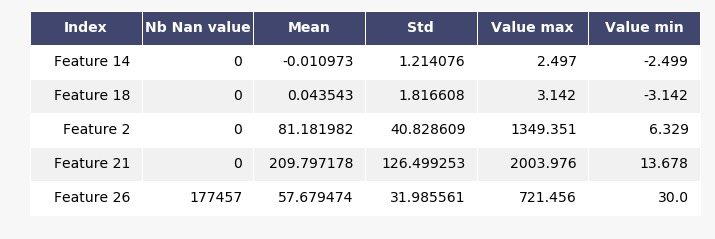
\includegraphics[width=\columnwidth]{features.png}
  \caption{Features Example}
  \vspace{-3mm}
  \label{fig:features}
\end{figure}

In order to better understand the interaction and dependencies between the features, it is interesting to output their scatter plot matrix, as shown in Figure ~\ref{fig:scatterplot}. The first observation from there is that a few of them are indeed correlated with clear shapes appearing on the plots. Then, their distribution can vary a lot, from being normally distributed to equally.

\begin{figure}[hbp]
  \centering
  \includegraphics[width=\columnwidth]{scatterplot_COLOR.png}
  \caption{Scatter Plot Matrix}
  \vspace{-3mm}
  \label{fig:scatterplot}
\end{figure}

\section{Feature Processing}

Our first results with the simple dataset were not sufficient. It was therefore decided to implement some processing in order to enhance our percentage of correct predictions. 

The first process was concerning the NaN values. A function nan\_handling can replace all the NaN values by our desired value, here a low negative value (A VERIFIER). Going through all the features, we try to apply different functions to the features: exponantial, cosinus, square root, logarithm and the power function. If the resulting feature present a better correlation, we keep it. 

Then, from the scatterplot matrix, we observe features that seem highly correlated; for example features 2 and 7. After that, we multiply them together and keep the resulting feature if the result is satisfying.

\section{Machine Learning Methods}

\section{Results}

\bibliographystyle{IEEEtran}
\bibliography{literature}

\end{document}
